\documentclass[a4paper, 12pt]{article}

\newcommand\tab[1][.6cm]{\hspace*{#1}}
\usepackage[brazil]{babel}
\usepackage[utf8]{inputenc}
\usepackage{amsmath}
\usepackage{mathtools}
\usepackage{indentfirst}
\usepackage{graphicx}
\usepackage{multicol,lipsum}
\usepackage{blindtext}
\usepackage{verbatim}
\usepackage{textcomp}
\usepackage{hyperref}
\usepackage{float}
\usepackage{url}
%\usepackage{sbc-template}

\begin{document}
%\maketitle

\begin{titlepage}
	\begin{center}
	
	\begin{figure}[ht]
    \centering
    
\includegraphics[width=.44\textwidth]{Images/LogoUFSJ.PNG}
    \label{fig:Capturar.PNG}
    \end{figure}

    	\Huge{Universidade Federal São João del Rei}\\
		\Large{Curso de Ciência da Computação}\\ 

        \vspace{110pt}
        \textbf{\LARGE{
        \\
        \\
        \\
        Trabalho Prático 1: Relatório\\
        \vspace{0.5cm}
        \Large{Mineração de Dados Aplicada}
        \\
        \\
        \\
        }}
        
		\title{{\large{Título}}}
		\vspace{2.5cm}
	\end{center}
	    
    \begin{flushleft}
		\begin{tabbing}
		\\
		\\
		\\	
		\large{Discente: Julio Cesar da Silva Rodrigues}\\
	    \\
		\large{Docente: Leonardo Chaves Dutra da Rocha}\\
	    \end{tabbing}
    \end{flushleft}
	\vspace{1cm}
	
	\begin{center}
		\vspace{\fill}
			Abril\\
		    2023
	\end{center}
\end{titlepage}

\tableofcontents
\newpage

\section{Introdução}

O acesso à internet e, por consequência, o acesso às URLs, pode pavimentar um caminho direto para ações maliciosas contra usuários com a ação de um simples clique. As ameaças são das mais diversas, desde infecções por tipos de \emph{malware}, até furto (ou roubo) de informações sensíveis.

Neste contexto, o objetivo deste trabalho se pontua a desenvolver um modelo para predições de tipos URLs, usufruindo de conceitos e tecnologias relacionadas à mineração e ciência de dados e aprendizado de máquina, percorrendo parcialmente ou totalmente o processo KDD. 

O foco principal se apresenta na engenharia de dados, na tentativa de extrair informações relevantes de uma base de dados extremamente compacta, com o intuito de obter bons resultados nas classificações.

\subsection{Base de Dados}

A base de dados escolhida contém informações sobre URLs maliciosas, mais especificamente a URL e seu tipo, ou seja, um atributo e uma classe. Tal base contém 651191 instâncias, e as classes para cada URL em texto puro presente na base, podem assumir quatro valores: \emph{benign}, \emph{defacement}, \emph{phishing} e \emph{malware}. A base de dados está disponível publicamente na plataforma \emph{Kaggle}, e pode ser acessada em: \url{https://www.kaggle.com/datasets/sid321axn/malicious-urls-dataset}.

Em uma análise inicial, podemos observar que a disparidade em relação a distribuição das instâncias por classe é grande (Figura \ref{fig:exampleFig1}), com a fração de URLs benignas quase alcançando os 70\% da totalidade. Isto já pode sugerir implicitamente, a possível aplicação de uma técnica para balanceamento da base, na tentativa de obter um modelo com melhor desempenho e mais confiável (menor viés).

\begin{figure}[H]
    \centering
    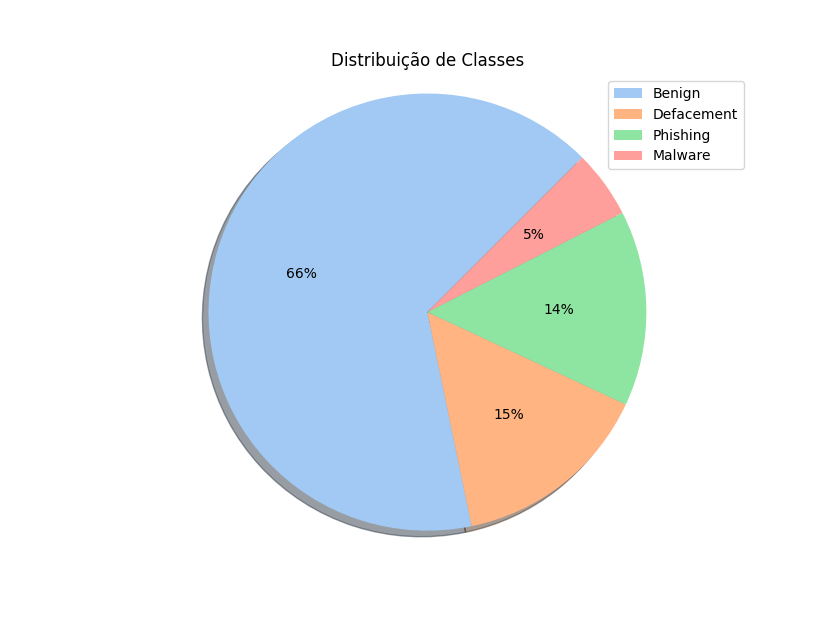
\includegraphics[width=1\textwidth]{Images/Figure_1.png}
    \vspace*{-1.8cm}
    \caption{Distribuição das classes na base de dados}
    \label{fig:exampleFig1}
\end{figure}

\section{Metodologia}

Nesta seção, será apresentado todo o percurso percorrido no desenvolvimento do trabalho. Serão citadas desde as tecnologias utilizadas na formulação da implementação, até detalhes em relação à distribuição dos dados da base, e como cada característica das URLs foi analisada e escolhida (ou não) para derivação em um atributo da base. 

Para o desenvolvimento deste trabalho, foi utilizada a linguagem \emph{Python} na implementação por completo. Particularmente, foram utilizadas as bibliotecas \emph{scikit-learn} e \emph{xgboost} na formulação dos modelos de aprendizado de máquina e aplicação de algumas técnicas de pré-processamento e validação. Também foi utilizada a biblioteca \emph{pandas} (em conjunto com \emph{scikit-learn}) para manipulação da base de dados. Por fim, foram utilizadas as bibliotecas \emph{Matplotlib} e \emph{seaborn} para visualização prática dos dados.

A implementação completa está disponível publicamente em: \url{https://github.com/juliorodrigues07/url_detection}. Para facilitar a visualização, um \emph{notebook} completo com as execuções pode ser acessado em: \url{https://colab.research.google.com/github/juliorodrigues07/url_detection/blob/sprint2/notebook/url_detection.ipynb}.

\subsection{Criação de Atributos}

Nesta subseção, será discutida a base central para o desenvolvimento deste projeto. O foco neste ponto, é a criação de novos atributos na tentativa de extrair informações úteis de URLs em texto puro, para então identificar padrões e possibilitar a classificação de tais instâncias. É importante citar que todo o processo de criação dos atributos ocorreu com base na execução de análises somente no que tange a estrutura da URL, ou seja, no escopo léxico das mesmas. A maior parte deste processo foi executada com a utilização de uma biblioteca dedicada para análise de URLs (\emph{urllib}) e expressões regulares.

O ponto de partida para criação de alguns dos atributos à serem apresentados, foi obtido a partir de uma exploração rápida de dois artigos relacionados à detecção de URLs maliciosas, estes que foram publicados na biblioteca digital \emph{IEEE Xplore} \cite{10019269} e \cite{9950508}. 

\subsubsection{Protocolo de Comunicação}

A primeira inspeção realizada nas instâncias presentes na base de dados, foi em relação ao protocolo de comunicação utilizado por cada página, cujo resumo gráfico pode ser observado na Figura \ref{fig:exampleFig2}. Constatou-se que o protocolo não é especificado na maioria das instâncias da base, enquanto uma fração de aproxidamente 25\% utiliza HTTP, e a porção restante (ainda menor, com 2,4\%) utiliza HTTPS.

Analisando mais detalhadamente, foi constatado que 85,7\% das URLs que utilizam o protocolo HTTP são maliciosas. Além disso, este conjunto de URLs maliciosas se divide apenas entre \emph{phishing} e \emph{malware}, ou seja, nesta base de dados, dada uma URL qualquer que utiliza o protocolo HTTPS, existe uma chance altíssima de que esta seja do tipo malicioso, mais especificamente, \emph{phishing} e \emph{malware}.

Ainda acerca dos protocolos utilizados, também foi observado que todas as instâncias pertencentes à classe \emph{defacement} utilizam o protocolo HTTP. Neste momento, podemos começar a formular hipóteses iniciais de que o protocolo de comunicação utilizado pode ter grande influência na classificação de URLs, e pode vir a tornar-se uma informação importante para ser extraída da base, e transformada em um atributo. 

\begin{figure}[H]
    \centering
    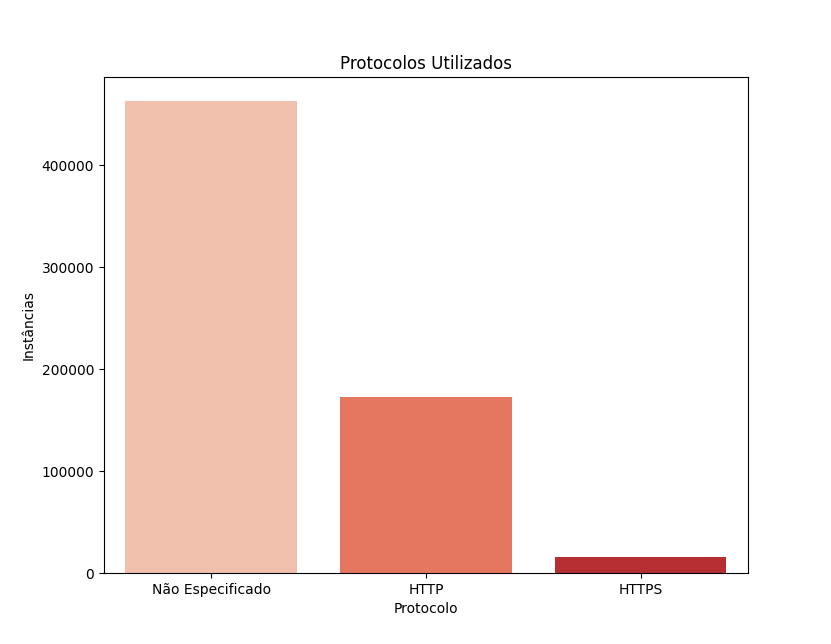
\includegraphics[width=1\textwidth]{Images/Figure_2.png}
    \caption{Distribuição de protocolos utilizados entre as URLs}
    \label{fig:exampleFig2}
\end{figure}

\subsubsection{Comprimento das URLs}

Outra característica analisada quanto às estruturas da URL, foi com comprimento em caracteres que cada uma apresenta (Figura \ref{fig:exampleFig3}). O motivo de analisar uma informação tão simples é de que, em muitos casos, URLs maliciosas tendem a possuir um tamanho acima da média para disfarçar possíveis informações suspeitas presentes no corpo da URL.

Analisando algumas estatísticas em relação às instâncias desta base de dados, foi observado que URLs de \emph{defacement} são, em média, 50\% maiores que URLs seguras, enquanto URLs de \emph{phishing} são, em média, 25\% menores que URLs seguras. Além disto, URLs que utilizam o protocolo HTTP e HTTPS, estas que possuem conjuntos consideráveis de URLs do tipo malicioso são, em média, de 63\% a 72\% maiores que as de protocolo não explícito. Todas estes aspectos influenciam na classificação de URLs de \emph{defacement}.

\begin{figure}[H]
    \centering
    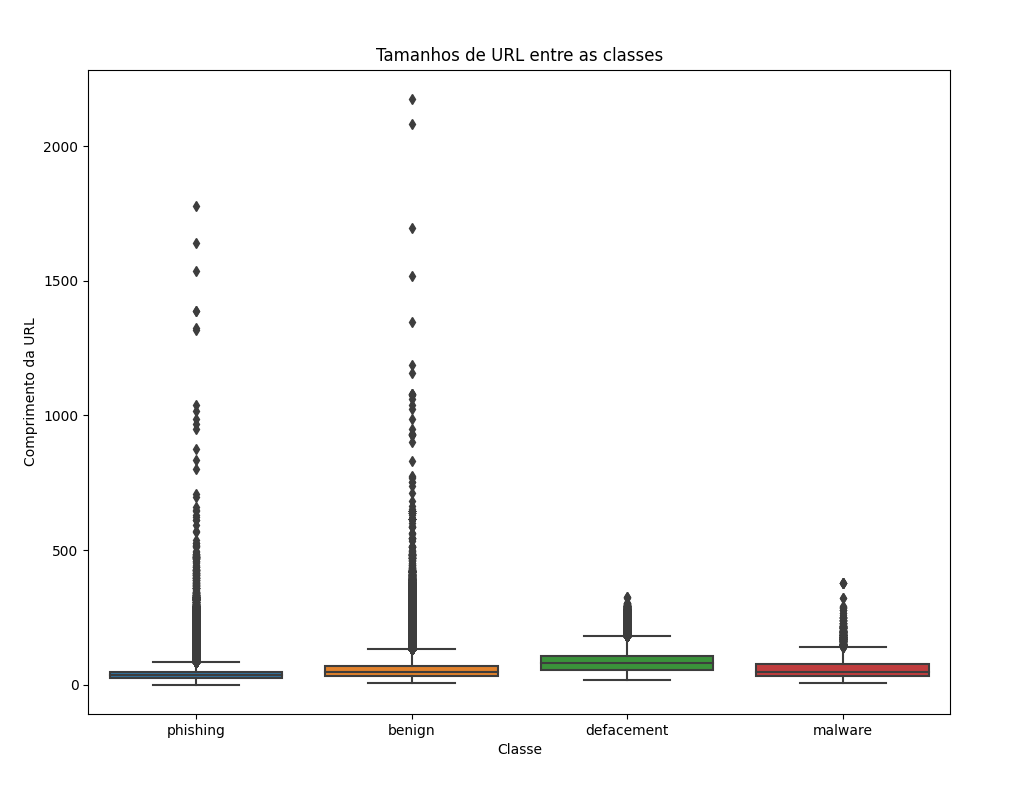
\includegraphics[width=1\textwidth]{Images/Figure_6.png}
    \caption{Distribuição de tamanhos de URL por classe}
    \label{fig:exampleFig3}
\end{figure}

Analisando o gráfico na Figura \ref{fig:exampleFig3}, podemos observar um conjunto relevante de \emph{outliers}, apresentando-se principalmente nos tamanhos de URLs dos tipos \emph{phishing} e \emph{benign}. Neste ponto, foi realizada uma análise acerca da distribuição dos tamanhos de URL em quartis na base de dados, obtendo algumas observações bastante relevantes.

Verificou-se que ao analisar o terceito quartil da base (Q3) ordenando-as de forma crescente pelo comprimento da URL, as 75\% menores URLs possuíam até 77 caracteres apenas, enquanto as 25\% maiores, distribuíam-se com tamanho variando na faixa de 77 as 2215 caracteres. 

Na tentativa de contornar este problema com \emph{outliers}, foi realizado o processo de \emph{equal-frequency binning} para distribuir a faixa de tamanhos das URLs somente entre quatro grupos de mesma quantidade (atributo com quatro valores), reduzindo bastante a faixa de valores e, por consequência, aumentando a ocorrência de padrões na base de dados.

No entanto, esta redistribuição dos dados não surtiu o efeito desejado. A faixa excessivamente longa (\emph{phishing} e \emph{benign}) se tornou um problema no processo de mapeamento do comprimento das URLs. Com a diferença de valores evidente entre o terceiro quartil e o restante da base, as faixas mapeadas foram bastante desproporcionais entre si. Outro ponto importante é que a faixa de valores original poderia ser um problema, mas para bases de dados pequenas. Com a faixa original, é perfeitamente possível encontrar padrões em uma base com centenas de milhares de instâncias.

\begin{figure}[H]
    \centering
    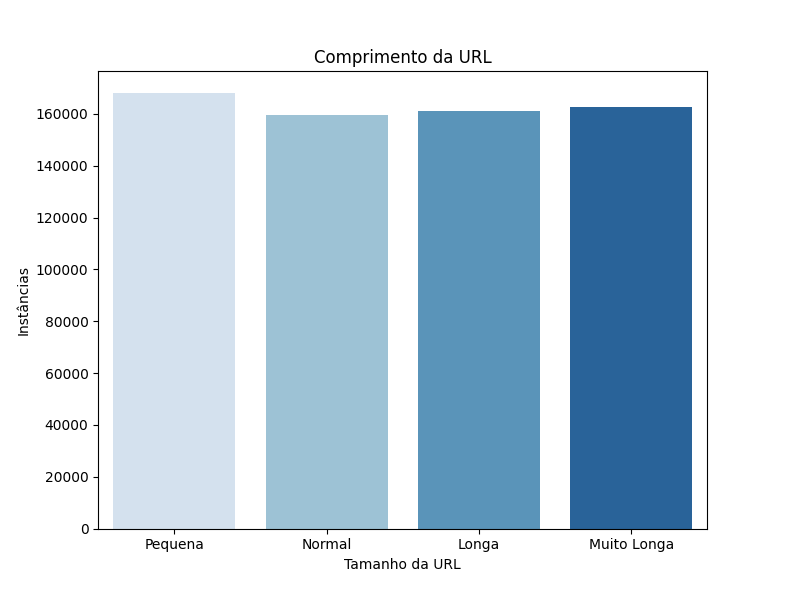
\includegraphics[width=1\textwidth]{Images/Figure_3.png}
    \caption{Aplicação de \emph{equal-frequency binning}}
    \label{fig:exampleFig4}
\end{figure}

\subsubsection{Atributos Estritos}

Dando sequência à análise estatística superficial do léxico das URLs da base de dados, foram notadas outras informações relevantes que culminaram para a criação de novos atributos. Em relação ao tamanho do primeiro diretório das URLs, URLs de \emph{malware} apresentaram, em média, tamanhos 50\% maiores que URLs seguras. Já o comprimento do primeiro diretório das URLs de \emph{phishing} é, em média, 25\% menor do que de URLs seguras.

Em relação à outro aspecto das estruturas das URLs, foi constatado que URLs de \emph{malware} possuem, em média, mais que o dobro de dígitos presentes em uma URL segura. No entanto, URLs de \emph{phishing} possuem, em média, 35\% menos dígitos que URLs benignas. A introdução de tais novos atributos fortaleceu o modelo na classificação de URLs de \emph{defacement} e \emph{phishing}, enquanto os ganhos para \emph{malware} apresentaram-se mais discretos.

\subsubsection{Palavras Suspeitas}

Por fim, foi criado um atributo baseado não em valores discretos, mas na ocorrência de cadeias de caracteres internamente ao texto da URL. Esta estratégia foi pensada na tentativa de destacar mais facilmente casos de URLs de \emph{phishing}, procurando por palavras como: \emph{free}, \emph{bonus}, \emph{account}, entre outras que poderiam estar indicando casos potenciais de roubo de informações sensíveis. Como será discutido mais adiante, o impacto no ganho de informação provido por este atributo foi mínimo, o que tornou sua presença na base apenas um adicional de custo computacional.

\section{Análise}

Nesta seção, serão realizadas algumas análises mais aprofundadas quanto à relevância de cada atributo criado na tarefa classificação no modelo, assim como alguns dados brutos da mesma.

\subsection{Relevância dos Atributos}

Finalizado o processo central do trabalho de criação de atributos, foi executada uma análise breve das relevâncias de cada um para o aprendizado do modelo. Para o algoritmo \emph{XGBoost}, podemos observar na Figura \ref{fig:exampleFig5} que o protocolo é evidentemente o atributo que mais fornece ganho de informação para o modelo, sendo responsável quase que por definir a classe conta própria.

Na Figura \ref{fig:exampleFig6}, é apresentada a importância de cada atributo no modelo de treinamento utilizando o algoritmo de regressão logística. Embora existam certas divergências entre o 2º e o 5º lugar (causados pela diferença no cálculo de relevância e até mesmo pelo algoritmo utilizado), o protocolo de comunicação utilizado é uma constante no aprendizado de ambos modelos, apresentando ganho de informação altíssimo. No lado negativo, o atributo de identificação de palavras suspeitas confirma sua baixa contribuição na classificação, apresentando-se em último lugar em relação à relevância para os modelos.

\begin{figure}[H]
    \centering
    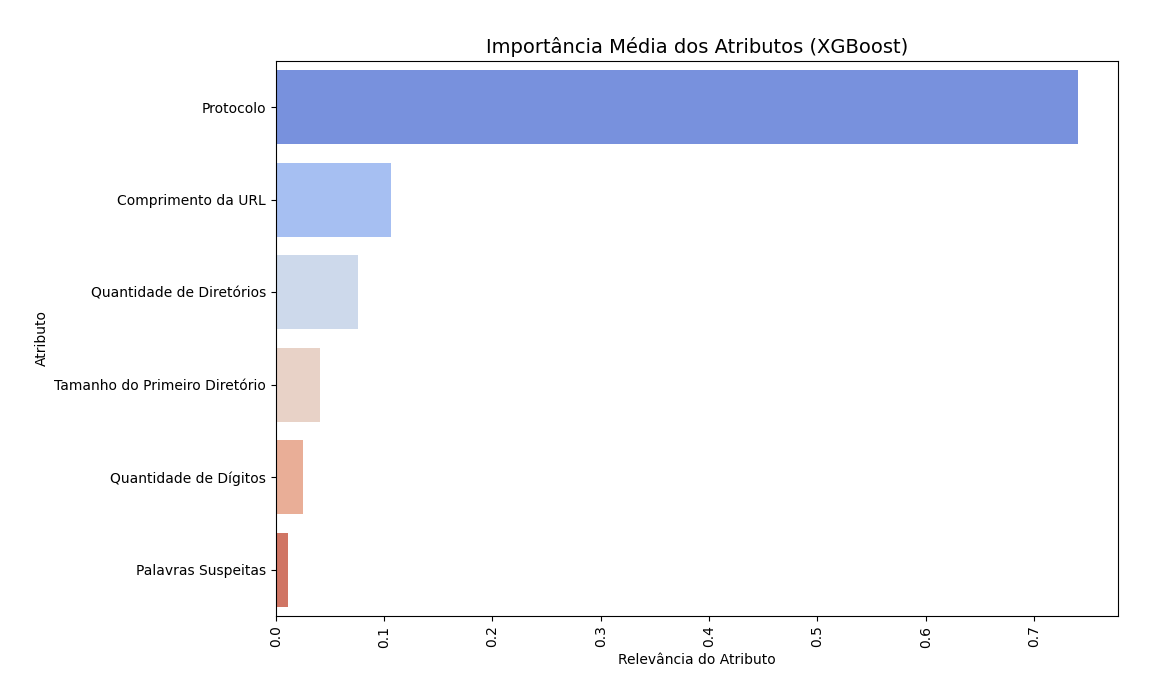
\includegraphics[width=1\textwidth]{Images/Figure_4.png}
    \caption{Relevância de cada atributo com \emph{XGBoost}}
    \label{fig:exampleFig5}
\end{figure}

\begin{figure}[H]
    \centering
    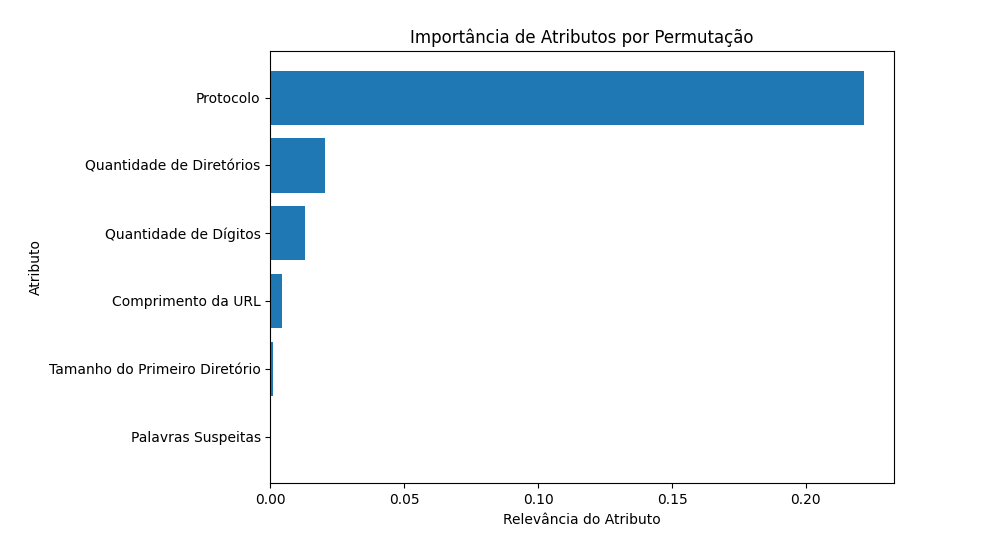
\includegraphics[width=1.1\textwidth]{Images/Figure_5.png}
    \caption{Relevância de cada atributo com Regressão Logística}
    \label{fig:exampleFig6}
\end{figure}

\subsection{Matriz de Confusão}

A matriz de confusão obtida na aplicação dos testes \emph{holdout} com o algoritmo \emph{XGBoost} é exibida na Figura \ref{fig:exampleFig7}. Podemos observar que em geral, o número de predições errôneas para cada classe não ultrapassa as mil unidades com 20\% da base de dados. No entato, o baixo resultado observado na \emph{F1-Score} para a classe \emph{malware} fica evidente, com mais de oito mil instâncias da mesma sendo classifcadas como seguras, a classe "rival". 

Tal resultado é alarmante, já que classificar instâncias com o tipo incorreto de URL maliciosa ou até mesmo classificar URLs benignas em maliciosas, possui um impacto sequer tão negativo quanto classificar URLs maliciosas como seguras.

\begin{figure}[H]
    \centering
    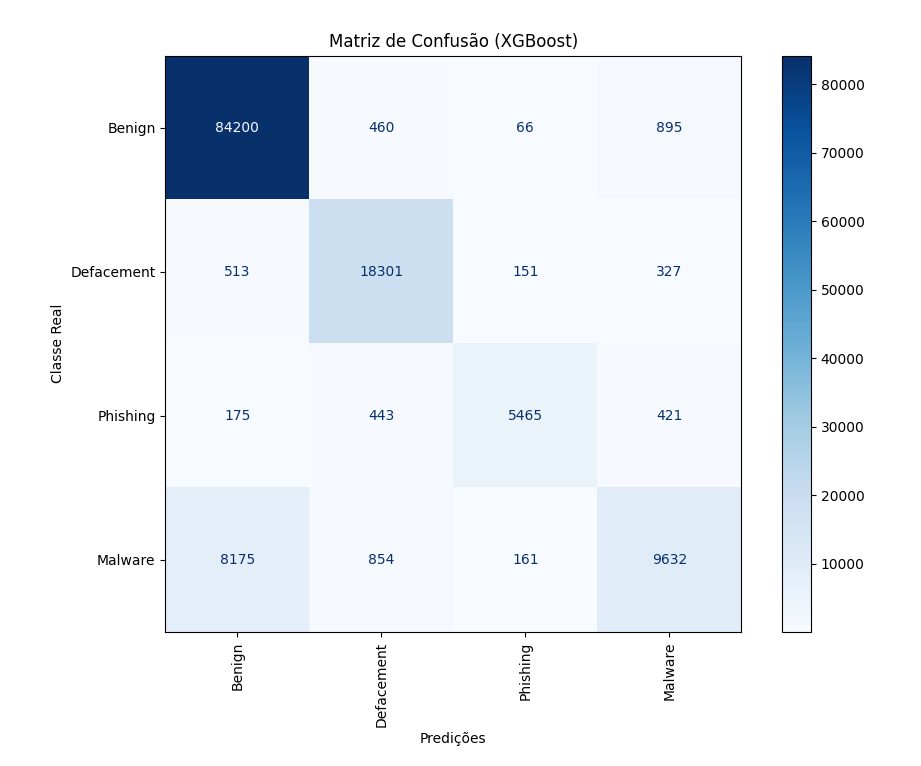
\includegraphics[width=1\textwidth]{Images/Figure_7.png}
    \caption{Matriz de confusão em teste com XGBoost}
    \label{fig:exampleFig7}
\end{figure}

\section{Resultados}

Nesta seção, serão apresentados de forma sumarizada, todos os resultados obtidos com a cosntrução dos modelos finais, minerando a base pré-processada com os novos atributos recém criados.

\subsection{Modelos de Aprendizado de Máquina}

Como o foco principal do trabalho se situa, quase que inteiramente, na etapa de preparação dos dados, somente foram selecionados dois métodos de aprendizado de máquina para trabalhar em cima da base de dados pré-processada. Adiantadamente, não foram realizados quaisquer processos de refinamento de hiperparâmetros do modelo ou experimentos com \emph{tripartite}.

Os algoritmos selecionados foram regressão logística e o \emph{XGBoost}. Enquanto a regressão logística é um algoritmo clássico, com princípio de funcionamento baseado em probabilidades, o XGBoost é um método \emph{ensemble}, isto é, utiliza um conjunto de vários algoritmos (neste caso, baseado em árvores de decisão) na tentativa de obter melhor desempenho preditivo, utilizando uma técnica de \emph{boosting}, a qual não será explanada neste trabalho.

À medida que os novos atributos foram criados, foram realizados testes \emph{holdout} (80\% para treinamento e 20\% para testes) de forma incremental, utilizando somente 5\% do total de instâncias da base para analisar rapidamente os ganhos (ou perdas). Na Tabela \ref{tab:exampleTab1}, pode ser observado o teste \emph{holdout} "final", utilizando a base por completo com os seis atributos criados.

\begin{table}[H]
    \centering
    \caption{Métricas obtidas com teste \emph{holdout} único}
    \vspace{0.3cm}
    \label{tab:exampleTab1}
    \begin{tabular}{c|c|c|c|c}
        \textbf{Class} & \textbf{Precision} & \textbf{Recall} & \textbf{F1-Score} & \textbf{Support}\\
        \hline
        Benign & 0.90 & 0.98 & 0.94 & 85621\\
        Defacement & 0.91 & 0.95 & 0.92 & 19292\\
        Phishing & 0.94 & 0.84 & 0.89 & 6504\\
        Malware & 0.85 & 0.51 & 0.64 & 18822\\
        \hline
        Accuracy &  &  & 0.90 & 130239\\
        Macro Avg & 0.90 & 0.82 & 0.85 & 130239\\
        Weighted Avg & 0.90 & 0.90 & 0.89 & 130239\\
    \end{tabular}
\end{table}

Os resultados obtidos utilizando a métrica \emph{F1-Score} foram aceitáveis para a maioria das classes. A única exceção foram as pontuações obtidas para as instância de \emph{malware}, que foram seriamente afetadas por sua menor presença (ou proporção) na base, além é claro, do efeito indesejedo na precisão do modelo, causado pela aplicação errônea da técnica de discretização não supervisionada (\emph{equal-frequency binning}) no atributo de comprimento das URLs.

\subsection{Validação Cruzada e Comparativos}

Para executar uma análise de maior credibilidade sobre o desempenho do modelo, foi utilizada a técnica de validação cruzada (\emph{k-fold}) com a base de dados recém processada, utilizando os dois algoritmos já citados. Os resultados obtidos podem ser observados na Tabela \ref{tab:exampleTab2}:

\begin{table}[H]
    \centering
    \caption{Métricas obtidas com validação cruzada (\emph{10-fold})}
    \vspace{0.3cm}
    \label{tab:exampleTab2}
    \begin{tabular}{c|c|c}
        \hline
        \multicolumn{3}{c}{\textit{Macro F1}}\\
        \hline
        \textbf{Modelo} & \textbf{Média} & \textbf{Desvio Padrão}\\
        \hline
        Regressão Logística & 0.4343240025832924 & 0.0014418608790156475\\
        XGBoost & 0.8218246353658317 & 0.001907892449405127\\
    \end{tabular}
\end{table}

É importante citar que tal técnica foi executada dividindo a base em dez partes (\emph{10-fold}). Além disso, os dados foram extraídos da base para cada bateria de treinamento-teste utilizando amostragrem estratificada, ou seja, todos os as parcelas (\emph{folds}) da base possuem a mesma distribuição (proporção) de classes da base original como um todo.

A métrica utilizada foi a \emph{Macro F1}, esta que é calculada para cada uma das classes, não levando em conta possíveis desbalanceamentos presentes na base de dados, o que é o caso afirmativo nesta base de URLs. Desta forma, a classe predominante (\emph{benign}), e que obteve os melhores resultados, não introduzirá viés no modelo, no caso da existência de outras classes com desempenho inferior.

O desvio padrão observado é mínimo em ambos os modelos, o que é um ótimo sinal de que a maiorias dos \emph{folds} representa de forma aceitável as nuâncias de todas as classes da base. Neste teste final, fica evidente que o XGBoost exige tempos maiores de processamento mas, em contrapartida, fornece os melhores resultados até o momento, mesmo existindo grandes margens para melhoria no processo KDD. 

\pagebreak

\section{Conclusão}

Em resumo, neste trabalho foi possível obter um primeiro contato com vários dos conceitos de mineração e ciência de dados, e aprendizado de máquina de forma prática, transitando nas etapas do processo KDD de forma superficial. 

Podemos observar a importância de se trabalhar o máximo possível com os dados antes de inferir quaisquer informações com a aplicação dos algoritmos. A aplicação incorreta ou incompleta de alguma(s) destas etapas podem produzir resultados negativos no modelo, levando à consequências enormes dependendo do contexto inserido.

\subsection{Passos Futuros}

Como próximos passos para prosseguir em um trabalho futuro com esta mesma base de dados, podemos citar a possibilidade de aplicar a extração de classes, unindo o conjunto \{defacement, phishing, malware\} em uma única classe (\emph{maliciosa}).

Na maioria dos casos, saber se um URL qualquer oferece risco de segurança basta para a maioria das finalidades. No entanto, para casos em que, por exemplo, deseje-se realizar alguma pesquisa ou apresentar alguma métrica sobre o tipo de novas URLs maliciosas identificadas, este modelo de classificação binária sofreria tal desvantagem com a perca de informação.

Outro ponto à ser expandido é a criação de novos atributos. Como citado anteriormente, os atributos foram criados somente analisando o léxico da URLs. Podemos expandir tais processos, analisando conteúdos da URL por exemplo, examinando o texto HTML das páginas e \emph{scripts} associados. Já em relação à rede, poderiam ser analisados aspectos como latência, número de portas abertas, DNS, entre outras características possivelmente agregadoras para o processo de classificação das URLs.

Por fim, poderia ser executado o processo de balanceamento da base para agregar confiabilidade ao modelo. Neste contexto, talvez poderia ser explorada a técnica de \emph{instance selection} com alguns testes iniciais para remover instâncias redundantes desta base volumosa, balanceado-a, reduzindo custo computacional e mantendo o desempenho do modelo ou até mesmo obter melhorias. Aplicados todos estes processos, poderia começar a bateria de ajustes finos para calibrar os hiperparâmetros ideias para o modelo.

\bibliographystyle{sbc}
\bibliography{ref.bib}

\end{document}
